\subsection{\rev{Test 1:} Lake-at-Rest Over an Uncertain Bed}

\rev{Numerical methods that are not well-balanced produce spurious waves in the vicinity of sloping topography, and these spurious waves are particularly evident for slow-moving flows with weak momentum fluxes.
In the limit, the momentum flux is zero and the water is motionless, like the water surface on a lake at rest.
Hence, the lake-at-rest test is ideally suited to verify the well-balanced property, since the analytic solution preserves the resting state forever, and any waves generated by a numerical model are entirely spurious.}

To present a challenging test, a rectangular obstacle is introduced to the right of the uncertain hump given by equation~\eqref{eqn:bed}, so the bed elevation $z$ becomes
\begin{subequations}
\begin{align}
    z(x, \hump) &= \hump \sech^2 \left( \frac{\pi x}{\lambda} \right) + \zrectbump(x) \text{,}
    %
    \intertext{where $\zrectbump$ is the rectangular obstacle:}
    %
    \zrectbump(x) &= \begin{cases}
    \humpmean & \text{if $30 < x \leq 40$,} \\
    0 & \text{otherwise}
    \end{cases}
\end{align}
\end{subequations}

Results of the well-balanced stochastic model are compared with those of a stochastic model having a centred difference approximation of the source term vector that does not exactly balance the numerical flux gradient.
The centred difference model is the same as the well-balanced stochastic model except for two changes.
First, numerical fluxes are calculated using the original, unmodified flow variables:
\begin{align}
	\riemannflux_{i+1/2}^{(n)} = \riemannflux \left(
	\sum_{p=0}^P \flow^-_{i+1/2,p} \pcbasis_p, 
	\sum_{p=0}^P \flow^+_{i+1/2,p} \pcbasis_p
	\right) \label{eqn:flux-centred}
\end{align}
Second, the ensemble average of the source term vector uses a centred difference approximation:
\rev{\begin{align}
    \Ensemble{\source_i \pcbasis_l} =
    \left[ 0, -g \sum_{p=0}^P \sum_{s=0}^P h_{i,p}
    \frac{z_{i+1,s} - z_{i-1,s}}{2 \Delta x}
    \Ensemble{\pcbasis_p \pcbasis_s \pcbasis_l} \right]^\T \label{eqn:source-centred}
\end{align}}
The centred difference model and the well-balanced model are both configured with a Wiener-Hermite basis order $P = 3$.

\begin{figure}
\centering
\begin{subfigure}{\textwidth}
\phantomsubcaption\label{fig:lakeatrest:centred:eta}
\phantomsubcaption\label{fig:lakeatrest:sgm:eta}
\phantomsubcaption\label{fig:lakeatrest:centred:q}
\phantomsubcaption\label{fig:lakeatrest:sgm:q}
\centering
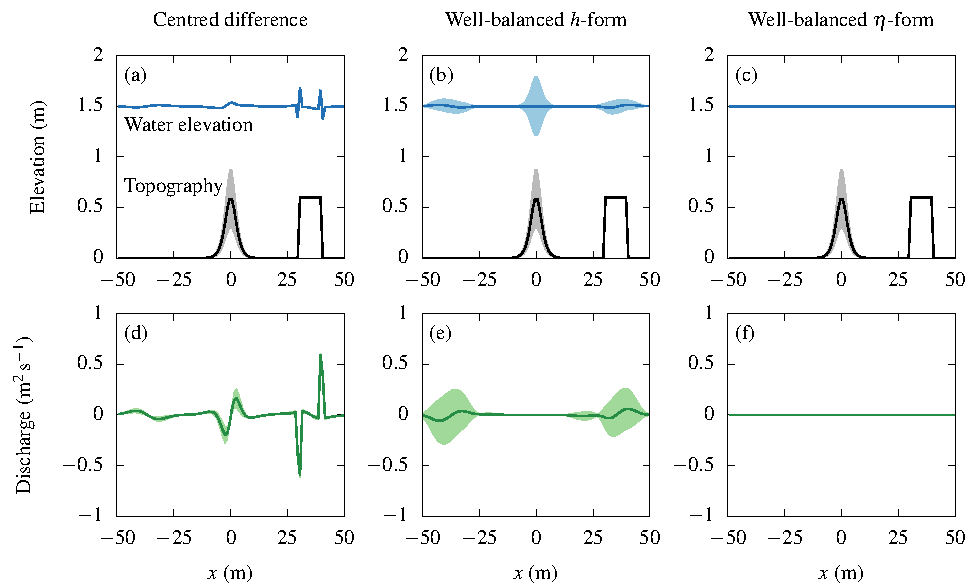
\includegraphics{fig-lakeatrest.pdf}
\end{subfigure}
\caption{Stochastic lake-at-rest solutions at $t = \SI{100}{\second}$.
Mean values are marked by solid lines and shaded regions represent one standard deviation from the mean.}
\label{fig:lakeatrest}
\end{figure}

The simulated time is \SI{100}{\second} corresponding to about 670 timesteps, and the solutions for the centred difference and well-balanced stochastic Galerkin models are shown in figure~\ref{fig:lakeatrest}.
The lack of well-balancing is apparent using the centred difference model: grid-scale standing waves develop at the discontinuities either side of the rectangular hump (figure~\ref{fig:lakeatrest:centred:eta}, \ref{fig:lakeatrest:centred:q}), and a smooth standing wave also develops over the uncertain hump.
These errors persist throughout the simulation.
In contrast, the well-balanced stochastic Galerkin model preserves the initial resting state with discharges accurate to machine precision (figure~\ref{fig:lakeatrest:sgm:q}).
This numerical result confirms that the stochastic Galerkin model is well-balanced in theory and in practice.

The choice of the Wiener-Hermite basis introduces a particular limitation that imposes an upper bound on the basis order $P$, and constrains the minimum water depth that the stochastic Galerkin model can represent.
This limitation arises because the hump amplitude has a Gaussian probability distribution so the tails of the distribution extend to $\pm \infty$, meaning that there is a non-zero probability that the water depth is negative.
The stochastic Galerkin formulation presented here does not accommodate wetting-and-drying processes, and any negative water depth will crash the model.
If the basis order $P$ is increased then the Gauss-Hermite quadrature points in equation~\eqref{eqn:pc-flux} extend further into the tails of the probability distributions, leading to negative water depths being provided as input to the Riemann solver.
Similarly, raising the topography, decreasing the initial water depth, or increasing the topographic uncertainty can all produce negative water depths in the stochastic Galerkin model.
This behaviour has been verified experimentally by varying the model basis order, initial conditions and topography profile.

